\documentclass[a4paper]{article}

\usepackage[utf8]{inputenc}
\usepackage[T1]{fontenc}
\usepackage{textcomp}
\usepackage[italian]{babel}
\usepackage{graphicx}
\usepackage{siunitx}
\usepackage{float}
\usepackage{amsmath, amssymb}

\sisetup{uncertainty-mode=separate}

\title{Relazione di Laboratorio - Conteggi}
\author{Walhout Francesco - Iallorenzi Michele}

\begin{document}
    \maketitle

    \section{Introduzione}
        In questa esperienza analizzeremo la lunghezza dei versi e la frequenza di una
        singola lettera all'interno dell'intero testo della \emph{Divina Commedia} di 
        Dante Alighieri. Lo scopo è ottenere dimestichezza con le distribuzioni
        univariate di base (binomiale, poissoniana, normale) e con il test del $\chi^2$.\\
        Non possiamo certo supporre che la lunghezza dei versi sia completamente casuale
        poiché il poema è stato scritto in endecasillabi, ovvero versi composti da $11$ 
        sillabe, tuttavia le sillabe posso variare di lunghezza e includeremo spazi e 
        punteggiatura nei nostri conteggi, quindi possiamo aspettarci una variazione
        casuale della lunghezza dei versi attorno ad una media che è invece determinata
        dalla scelta stilistica dell'endecasillabo.
    \subsection{Strumenti utilizzati}
    \begin{itemize}
        \item Una copia digitale della  \emph{Divina Commedia} di Dante Alighieri.
        \item Un computer capace di eseguire i conteggi e l'analisi dati necessari.
    \end{itemize}

    \section{Misure ed Analisi}
    \subsection{Conteggi}
        Abbiamo scelto di eseguire il conteggio attraverso un programma in python, questo
        ci ha permesso di analizzare l'intera opera, ma un analisi simile può essere fatta
        a mano su una porzione molto più piccola del testo.
        Come anticipato abbiamo contato il numero di caratteri di ciascuno dei
        versi, contando lettere, spazi e segni di punteggiatura.
        Abbiamo inoltre contato il numero di occorrenze della lettera "a" in ciascun
        verso; sia le maiuscole che le minuscole sono state contate, ma non le lettere 
        accentate.
    \subsection{Elaborazione dei dati}
        Dopo aver ottenuto una lista contenente la lunghezza $l_i$ di ciascuno dei
        $N_v=14233$ versi, abbiamo realizzato un istogramma con un canale per ciascuna
        lunghezza (mostrato in figura \ref{fig:lunghezze_versi}) ed abbiamo cercato di
        verificare l'ipotesi che questi dati si distribuissero secondo una poissoniana
        o secondo una gaussiana.\\
        Per farlo abbiamo innanzi tutto sovrapposto i grafici delle occorrenze attese
        secondo queste due distribuzioni all'istogramma di cui sopra. In particolare le funzioni
        utilizzate rispettivamente per la distribuzione poissoninana e per la distribuzione
        gaussiana sono:
        \begin{gather}
            \mathcal{P}\left( k;\mu \right) = \frac{\mu^{k}}{k!}e^{-\mu} \label{eq:poisson}\\
            \mathrm{N}(k; \mu, \sigma) = \frac{1}{\sigma \sqrt{2 \pi} } e^{-\frac{1}{2}\left( \frac{k-\mu}{\sigma} \right)^2 } \label{eq:norm}
        \end{gather}
        Dove $k$ è la variabile aleatoria, mentre $\mu$ e $\sigma$ sono il valore atteso
        e la deviazione standard delle distribuzioni. Per questi due valori abbiamo
        utilizzato la media campione delle lunghezze $m = 35.9$ e la varianza campione
        delle stesse $s = 3.3$ ottenute tramite le relazioni:
        \begin{gather}
            m = \frac{1}{N_v}\sum_{i=1}^{N_v} l_i\label{eq:media}\\
            s = \frac{1}{N_v-1}\sum_{i=1}^{N_v} \left( l_i-m \right) ^2\label{eq:deviazione_standard}
        \end{gather}
        Moltiplicando le equazioni \ref{eq:poisson} e \ref{eq:norm} per il numero di versi
        $N_v$ si ottengono le distribuzioni mostrate in figura \ref{fig:lunghezze_versi}.\\
    \begin{figure}[ht!]
        \centering
        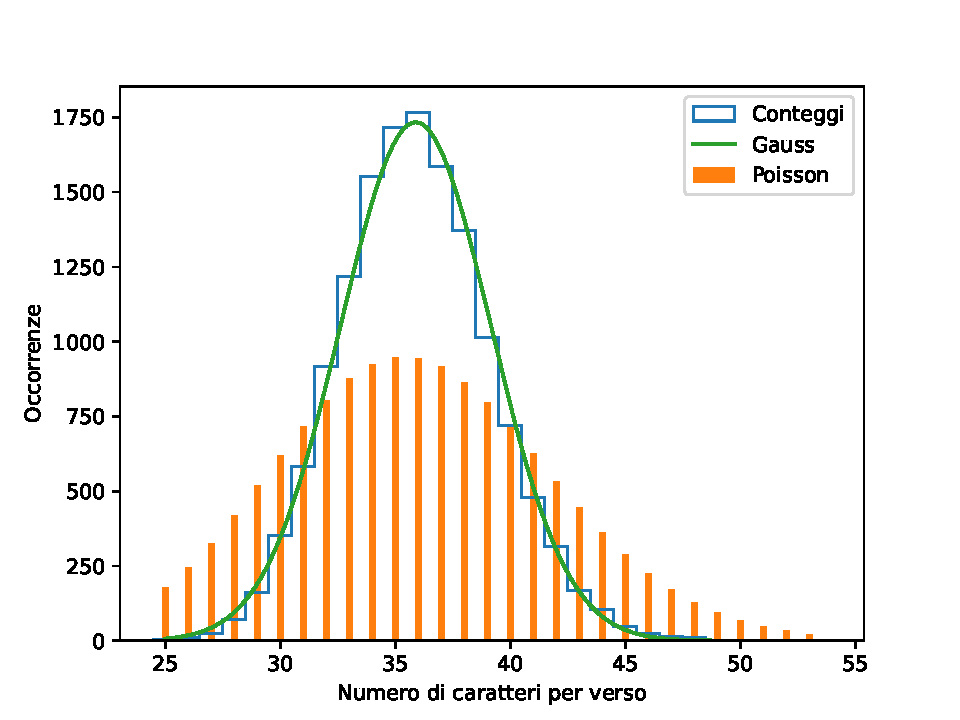
\includegraphics[width=0.8\textwidth]{extra/lunghezze_versi.pdf}
        \caption{Istogramma delle lunghezze dei versi sovrapposto ai valori attesi secondo
        le distribuzioni poissoniana e gaussiana.}
        \label{fig:lunghezze_versi}
    \end{figure}
        Per i conteggi delle occorrenze della lettera "a", abbiamo eseguito un procedimento
        analogo, ma utilizzindo invece la distribuzione poissoniana e quella binomiale,
        secondo la formula seguente:
        \begin{equation}
            \mathcal{B}(k;n,p) = \binom{k}{n}p^{k}\left( 1-p \right) ^{n-k}\label{eq:binom}
        \end{equation}
        Dove $k$ è ancora una volta la variabile aleatoria mentre per il parametro $p$ 
        abbiamo utilizzato il rapporto tra il numero totale di occorrenze della lettera
        "a" e il numero totale di caratteri e per il parametro $n$ abbiamo
        utilizzato la lunghezza media di un verso $m$ calcolata con l'equazione \ref{eq:media}.\\
        Per il parametro $\mu$ dell'equazione \ref{eq:poisson} in questo caso abbiamo utilizzato
        il valore $p\cdot m$. I grafici ottenuti sono mostrati in figura \ref{fig:frequenza_a}.\\
    \begin{figure}[ht!]
        \centering
        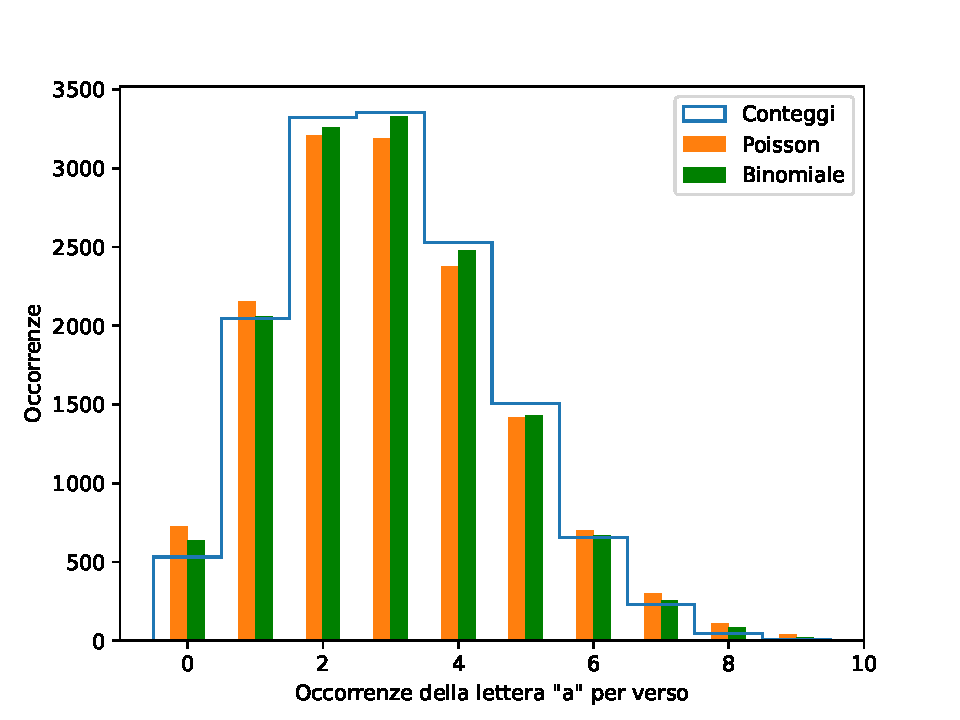
\includegraphics[width=0.8\textwidth]{extra/frequenza_a.pdf}
        \caption{Istogramma delle occorrenze per verso della lettera "a" sovrapposto ai valori
        attesi secondo le distribuzioni poissoniana e binomiale.}
        \label{fig:frequenza_a}
    \end{figure}
        Infine abbiamo ulteriormente verificato la validità delle ipotesi che i dati seguano ciascuna
        di queste distribuzioni attraverso dei test del $\chi^2$. 
        Le formule utilizzate per calcolare il $\chi^2$, la relativa deviazione standard
        $\sigma_{\chi^2}$ ed il numero di gradi di libertà $\nu$ sono:
        \begin{gather}
            \chi^2=\sum_{i=1}^{N_v} \frac{\left( o_i - e_i \right)^2 }{e_i}\\
            \sigma_{\chi^2} = \sqrt{2\nu} \\
            \nu=N_c-n_p-1
        \end{gather}
        Dove $o_i$ sono le occorrenze nell'i-esimo canale dell'istogramma in considerazione,
        $e_i$ sono i valori attesi da ciascuna distribuzione per l'i-esimo canale dell'istogramma,
        $N_c$ è il numero di canali dell'istogramma e $n_p$ è il numero di parametri per ciascuna distribuzione ($1$ per la
        poissoniana e $2$ per la gaussiana e la binomiale).\\
        I valori attesi $e_i$ nel caso della distribuzione poissoniana e binomiale sono
        rispettivamente $N_v \cdot  \mathcal{P}(k_i;\mu)$ e $N_v \cdot  \mathcal{B}(k_i, n, p)$,
        dove $k_i$ è la lunghezza dei versi nell'i-esimo canale dell'istogramma.\\
        Invece per la distribuzione gaussiana i valori attesi sono $N_v \cdot \int_{k_i}^{k_{i+1}} \mathrm{N}(x;\mu,\sigma)dx $
        dove gli estremi dell'integrale coincidono con gli estremi dell'i-esimo canale
        dell'istogramma.\\
        I valori ottenuti sono mostrati in tabella \ref{tab:chi2}.
        \begin{table}[ht!]
            \centering
            \label{tab:chi2}
            \begin{tabular}{c|c||c}
                \multicolumn{3}{l}{Lunghezza dei versi}\\
                \hline
                & Poissoniana & Gaussiana\\
                \hline
                $\chi^2$ & 5492.8 & 571.6\\
                $\nu$ & 27 & 26\\
                $\sigma_{\chi^2}$ & 7.3 & 7.2\\
                \hline\hline
                \multicolumn{3}{l}{Frequenza della lettera "a"}\\
                \hline
                & Poissoniana & Gaussiana\\
                \hline
                $\chi^2$ & 159.8 & 50.2\\
                $\nu$ & 8 & 7\\
                $\sigma_{\chi^2}$ & 4.0 & 3.7
            \end{tabular}
            \caption{caption}
        \end{table}
    \section{Conclusioni}
    Per le caratteristiche della distribuzione del $\chi^2$ ci aspettiamo che i valori di
    $\chi^2$ siano vicini al numero di gradi di libertà, questo però non avviene in nessuno
    dei test effettuati, infatti nel migliore dei casi i valori di $\chi^2$ e $\nu$ distano di 
    più di $11\sigma$.
    Possiamo quindi senza ombra di dubbio escludere che la lunghezza dei versi o la frequenza
    della lettera "a" seguano alcuna delle distribuzioni prese in analisi.\\
    Tuttavia possiamo dire che la distribuzione poissoniana comporta un errore maggiore
    per entrambi i dataset in analisi, mentre i valori attesi dalla distribuzione
    gaussiana e da quella binomiale sono notevolmente più vicini ai valori effettivi,
    tanto che un analisi svolta su una porzione minore di test potrebbe non essere stata
    sufficiente a smentire l'ipotesi nulla.
\end{document}
